\chapter{Сетевая коммуникация}\label{ch:ch3}

\subsubsection{3.1.1}

Recently, communication scholars have paid attention to the growing dissonant and dissipative character of the public spheres, especially in their connection to networked discursive spaces. While substantial dissonance of the discussions is well addressed, structural discontinuity of public discussion remains under-explored. Reproducibility of the discussions on similar issues or events in time, we argue, needs to be seen as a marker of stability of public spheres. In this paper, we compare the user and influencer structure of two similar discussions on German Twitter of 2016 (the Cologne mass harassment) and 2019 (the Chemnitz killing). We show that the overall reproducibility of the discussions is extremely low, and the only structural element that reproduces are influential media, mostly of national reach. But even the stability of media presence must be questioned, as both intensity of their presence within the discussion and user engagement with their tweets varies much from one discussion to the other. Thus, one may conclude that the structural stability of public discussion of similar events on Twitter is not reached.

\subsubsection{3.2.1}

Предметом исследования является использование пиктограмм для выражения эмоций и чувств в сетевой коммуникации. Объектом исследования выступили комментарии в нескольких популярных у молодежи сообществах социальной сети «ВКонтакте». Целью исследования было сравнение предпочитаемых пиктограмм-эмодзи, которыми выражают свои эмоции и чувства пользователи, состоящие в сообществах с разной частотой использования обсценной лексики. Гипотезой исследования выступило предположение, что группы с разной частотой использования обсценной лексики отличаются эмоциональной тональностью и используемыми пиктограммами-эмодзи для выражения эмоций и чувств. Методами исследования выступили опрос и контент-анализ. Для реализации первого метода была составлена анкета, в которой респондентам были заданы вопросы об особенностях их интернет-предпочтений, наиболее привлекательных для них интернет-сообществах в социальных сетях. Проведен анкетный опрос на выборке 854 человека, осуществлен сбор данных о частотности использования пиктограмм-эмодзи в 14 выделенных для детального анализа сообществах социальной сети ВКонтакте. Выявлено, что в сообществах, где пользователи реже используют ненормативную лексику, рейтинг эмодзи, обозначающих положительные (гедонические и сближающие) эмоции выше. В сообществах, где нецензурная брань используется чаще, пользователи наравне с позитивными, часто используют пиктограммы выражающие негативные эмоции -- удаляющие (гнев, злость) и меланхолические (печаль, тоска). Результаты исследования могут быть применены в разработке методов мониторинга настроений участников сетевой коммуникации.

\section{Принципы взаимодействия и распространения информации}\label{sec:ch3/sec1}

\subsection{Discontinued Public Spheres? Reproducibility of User Structure in Twitter Discussions on Inter-ethnic Conflicts}\label{subsec:ch3/sec1/sub1}

\subsubsection{1. Introduction}\label{subsubsec:ch3/sec1/sub1/subsub1}

Recently, communication scholars have stated that today’s public spheres \cite{Habermas} have become increasingly dissonant \cite{Pfetsch} and disintegrated. They rarely have consensus as a goal and, to a large extent, consist of ad hoc discussions \cite{BrunsBurgess} that have no continuity and quickly dissipate. Disconnection also emerges through ‘ever-more-fiercely negative campaigns, increasing political polarization, and public debates filled with prejudices and false assumptions’ \cite[p.~59]{Pfetsch}. One dimension of this disintegration has remained virtually unexplored, which is time. In traditionally mediated public spheres \cite{Calhoun}, the main structure of information flows organized by media and institutions remained stable in years or even decades; but we hardly know whether the user and influencer structure of networked discussions remains stable or changes with time, and to what extent. How can we expect public discussions to come to definitive conclusions stably accepted or at least discussed, if the very participant structure is unstable?

We argue that reproducibility of the discussion structure may be viewed as a sign of the long-term continuity of the public spheres and, thus, work as their quality metric. Long-term studies of networked discussions (\textit{e.g.} their polarization) remain rare despite the measurement’s tools accessible at the platform such as networking, tweeting and content-producing behavior of users \cite{GarimellaWeber}. ‘Most longitudinal network studies have confounded the processes of new tie formation and old tie maintenance, resulting in an incomplete understanding of the processes of network change’ \cite{Fu}. Studying Twitter data in timelines and investigating timeline narratives longitudinally are, till today, atypical approaches to data gathering and analysis \cite{BrookerVinesBarnett}; comparisons between structures of similar discussions of various times are next-to-absent.

Conflictual discussions online are vivid forms of expression of the public sphere \cite{BodrunovaBlekanovSmoliarova}. Among them, Twitter discussions are the most rapidly growing and, sometimes, most quickly dissipating. Our previous findings have shown that Twitter ‘is more complicated than the imaginary cocooned talk in echo chambers, especially for issues beyond elec- tions and direct policing’ \cite[p.~130]{BodrunovaBlekanovSmoliarova}. Moreover, according to the studies of digital protest and ‘hashtag activism’, Twitter may enable longitudinal campaigning that changes structure and content of public discussions for long enough time periods \cite{BonillaRosa}. Technological affordances equally contribute to the formation of social movements and the spread of false beliefs in the ‘unedited public sphere’ \cite{BimberDeZuniga} that emerges on social media. They also simultaneously allow for keeping the talk alive and forgetting it as soon as it goes beyond the Twitter scroll.

Case studies of Twitter discussions on selected conflicts paid more attention to the content of debate and the character of public communication than to who and how long participates in the discussion \cite{GroshekTandoc}. Also, comparative approaches have mostly been applied to simultaneous cases in different countries, not to similar discussions that hap- pened within one national context in varying times, with few exceptions when the scholars talk about a social/political movement with its evolving dynamics of activities (e.g. \#blacklivesmatter).

This study aims at comparing two national-level discussions in German-language Twitter about ethnicity-related conflicts: the one on the 2016 New Year’s Eve sexual assaults in Cologne and that on the 2018 protests in Chemnitz that took place after the death of a Cuban-German man. We ask to what extent the structure of influencers (ordinary users, media, and institutions) has remained similar, since the issue and public polarization behind it were the same. Comparison within the national context reduces bias present in cross-national studies, as the variety of influencers cannot be explained by varying national political cultures.

The structure of this paper is organized as follows. The next sections presents our research questions and methodology (Sect.~2) and the findings of our study (Sect.~3). We conclude with a short summary of our results (Sect.~4).

\subsubsection{2. Research Questions and Methodology}

As stated above, the study aims at comparing two national-level discussions in German- language Twitter about ethnicity-related conflicts: the one on the 2016 New Year’s Eve sexual assaults in Cologne and that on the 2018 protests in Chemnitz that took place after the death of a Cuban-German man. Our general assumption is that the structure of participation, as well as the structure of influencers, should remain similar, as the issue and public polarization behind the discussions were the same.

We conducted vocabulary-based web crawling to collect the discussion content and to analyze their structure. A special web crawler has been developed to bypass the limitations of Twitter API \cite{BlekanovSergeevMartynenko}. The total number of users in the two datasets included 12,382 users for Cologne and 22,973 users for Chemnitz.

As we moved from step to step in our research, we corrected the research questions and hypotheses based on the findings of the previous steps. Here, we will describe the RQs and methods used for each step, but the hypotheses are attached to the description of our results.

\paragraph{RQ1. Did Twitter users who discussed the Cologne case join the Twitter discussion about the Chemnitz case?}

To answer RQ1, we assessed the general reproducibility of the discussions by defining the number of all users and influencers who participated in both discussions.

\paragraph{RQ2. Does the structure of politically relevant (institutionalized political, grassroots political, and media) influencers repeat from Cologne to Chemnitz?}

To answer RQ2, we assessed the structure of influencers. For this, we sampled 50 top users for each of eight user metrics: number of tweets; number of interactions (likes, comments, and retweets); centralities "--- indegree, outdegree, betweenness, and pagerank. Then we merged them in aggregate lists of top users and eliminated the duplicates. As many users were within the top lists by many metrics, the final top lists included 230 users for the Cologne case and 207 users for the Chemnitz case. We manually coded the users in the final lists for their offline status in the following way. We coded an account as ‘ordinary user’ if its owner mentioned neither an institutional status nor political positioning in the user self-description at the top of the Twitter blog. If any political positioning or support of political values have been mentioned in the description, the account has been coded as ‘politically active blogger/activist.’ As ‘media’ we coded the accounts that either have a clear connection to a media project outside Twitter or position themselves as Twitter-only media projects. Institutional political actors included the accounts run by state authorities of any level and their individual representatives; political parties; individual politicians. Any other possible classification based on the description in the user account was marked as ‘other’.

\paragraph{RQ3. Does the salience of intersecting influencers differ in the two cases?}

To answer RQ3, we have defined the list of relevant intersecting influencers and have calculated their activity ratio and user engagement ratio. The former is the number of tweets published by the account in the first case divided by the number of tweets published in the second case; the latter is the ratio of the according numbers of user comments.

These ratios show whether the status of these influencers, both actively pursued and user-supported, has been stable in time.

\subsubsection{3. Findings}

\paragraph{3.1 Reproducibility of the General User Structure in the Discussions}

\paragraph{RQ1. Did Twitter users who discussed the Cologne case join the Twitter discussion about the Chemnitz case?}

\begin{itemize}
	\item H1a. \textit{Ad hoc} publics that emerged around the Cologne and Chemnitz cases repeat to a significant share (over 30\% of the participants who discussed Cologne also discussed Chemnitz).
	\item H1b. The list of top users changed less than the general sample of users taking part in the discussion, as influencers are the structural carcass of the issue-based debates.
\end{itemize}

To prove H1a we compared two general samples crawled for the Cologne case and for the Chemnitz case. From the whole dataset, we excluded those users who have not posted at least once and only interacted with those who tweeted by liking or sharing. (These users were crawled because they were necessary for the graph reconstruction of the discussions; we consider them irrelevant for RQ1.) The datasets for RQ1 included 12,382 users who tweeted about Cologne and 22,973 users who tweeted about Chemnitz. Only 1,735 users (circa 14\% of Cologne sample and 7,5\% of Chemnitz sample) participated in both discussions posting at least one tweet with at least one hashtag that defines the corpora of each discussion. 17\% of them published the same amount of posts (from 1 to 7 tweets in each discussion), 57\% tweeted more about Cologne and 26\% were more active in posting about Chemnitz. The total number of unique users amounts to 33,620 users; thus, the share of intersecting users is 5,2\%. If we exclude those who posted less than three tweets in both cases, the share of users participated in both discussions decreases even to 1,2\%. Therefore, H1a has to be rejected: the \textit{ad hoc} publics the emerged around the Cologne and Chemnitz events vary by 95\%.

To check H1b, we selected the top users (influencers) for both cases by the aforementioned procedure, which resulted into 222 users for the Cologne case and 207 users for the Chemnitz case, 413 unique users in total. Only 16 top users "--- 7\% from the Cologne top list and 7,7\% from the Chemnitz top list "--- have participated in both discussions (3,9\% of the total number of unique users; for the accounts, see Table~\cref{tab:intersectingInfluencers}). This also means that the list of top users changed slightly more than the general sample, but the difference seems not to be incredibly significant. Thus, H1ba is rejected, too.

\begin{table} [htbp]%
	\centering
	\caption{Intersecting influencers.}%
	\label{tab:intersectingInfluencers}% label всегда желательно идти после caption
	\renewcommand{\arraystretch}{1.5}%% Увеличение расстояния между рядами, для улучшения восприятия.
	\begin{SingleSpace}
		\begin{tabulary}{\textwidth}{@{}>{\zz}L >{\zz}C >{\zz}C@{}} %Вертикальные полосы не используются принципиально, как и лишние горизонтальные (допускается по ГОСТ 2.105 пункт 4.4.5) % @{} позволяет прижиматься к краям
			\toprule     %%% верхняя линейка
			Institutional type & Accounts & Number of users \\
			\midrule %%% тонкий разделитель. Отделяет названия столбцов. Обязателен по ГОСТ 2.105 пункт 4.4.5
			National media & BILD, DLFNachrichten, faznet, ndaktuell, SPIEGELONLINE, SZ, tagesschau, tazgezwitscher, welt, ZDFheute, zeitonline & 11 \\
			Regional media & WDR and ZDFnrw & 2 \\
			Journalists & MatthiasMeisner & 1 \\
			Bloggers & Korallenherz & 1 \\
			Politicians & HeikoMaas & 1 \\
			\bottomrule %%% нижняя линейка
		\end{tabulary}%
	\end{SingleSpace}
\end{table}

\paragraph{3.2 Reproducibility of the Influencer Structure: Politicization and Political Polarization}

\paragraph{RQ2. Is the structure of politically relevant (institutionalized political, grassroots political, and media) users among the influencers similar in both cases?}

\begin{itemize}
	\item H2a. The media segment of the influencer structure is the most stable (as media are the key actors in the mediated public sphere).
	\item H2b. The political segment (both institutional and grassroots) is more salient in the Cologne case (due to the political resonance of the case) (Table~\cref{tab:influencerCharacter}).
\end{itemize}

\begin{table} [htbp]%
	\centering
	\caption{Institutional character of influencers.}%
	\label{tab:influencerCharacter}% label всегда желательно идти после caption
	\renewcommand{\arraystretch}{1.5}%% Увеличение расстояния между рядами, для улучшения восприятия.
	\begin{SingleSpace}
		\begin{tabulary}{\textwidth}{@{}>{\zz}L >{\zz}C >{\zz}C@{}} %Вертикальные полосы не используются принципиально, как и лишние горизонтальные (допускается по ГОСТ 2.105 пункт 4.4.5) % @{} позволяет прижиматься к краям
			\toprule     %%% верхняя линейка
			Institutional type & Cologne & Chemnitz \\
			\midrule %%% тонкий разделитель. Отделяет названия столбцов. Обязателен по ГОСТ 2.105 пункт 4.4.5
			Institutional political actors & 5,22\% & 14,98\% \\
			Media & 23,48\% & 24,15\% \\
			Activists and politically active bloggers & 11,26\% & 27,05\% \\
			Ordinary & 50,00\% & 18,36\% \\
			Other/irrelevant & 11,74\% & 14,49\% \\
			Total N & 230 & 207 \\
			\bottomrule %%% нижняя линейка
		\end{tabulary}%
	\end{SingleSpace}
\end{table}

H2a is fully supported: the share of media accounts in both cases remained the same. Moreover, as shown in Table~\cref{tab:intersectingInfluencers}, 13 out 16 users that were high-ranked in both discussions are editorial mass media that operate mostly on the national level in Germany.


As for H2b, our findings demonstrate that political actors were much more visible in the discussion around events in Chemnitz that in Cologne: the share of institutionalized politicians has almost tripled. One might explain this tendency by the growth of Twitter activity of German politicians in general. SPD, die Linke, and FDP, as well as AfD, were fighting for users’ attention and gaining authority in an online discussion.

The salience of the AfD representatives has doubled. Four members of the right-wing party are present among the high-ranked users driving Twitter-discussion about events in Cologne in 2016, among them Björn Höcke, one of the founders of AfD Thuringia, the speaker of the parliamentary group of the AfD and the spokesman of the Thuringia Regional Association. In the discussion about Chemnitz in 2018, 8 accounts associated with AfD are found on the list of top users. All of them are ranked high by pagerank; 4 of 8 accounts are also ranked high by indegree and 1 by retweets.

Also, the rise of the grassroots politicization is clear. In our previous research on the Cologne case, we have shown that ‘many ordinary users have a clear political position that can be understood from their tweets, but they don’t define themselves as activists’ \cite[p.~141]{SmoliarovaBodrunovaBlekanov}. The Chemnitz case shows a clear difference: the share of ordinary people who explicitly declare their political position or another official status in their account descriptions has increased from 11\% to 27\%. This is another sign of politicization and political polarization during the case, as well as the sign of structural instability. Thus, H2b has not been supported.

\paragraph{3.3 Reproducibility of Intersecting Users and Their Roles: Media as the Carcass of Networked Discussions}

\paragraph{RQ3. Does salience of the intersecting accounts differ in the two cases?}

\begin{itemize}
	\item H3a. The activity ratios of the intersecting users remain stable (in between 0,8 and 1,2).
	\item H3b. The user engagement ratios of the intersecting users remain stable (in between 0,8 and 1,2).
\end{itemize}

We have shown above that media influencer accounts were, en masse, the only group of influencers that stably repeated in the two discussions. Hence, we have decided to assess the 13 media accounts that were discovered in both top user lists in terms of their activity and user engagement ratios.

Almost all media outlets tweeted more about Cologne than about Chemnitz (see Table~\cref{tab:mediaInfluencerRatios}). For public service TV, the difference is the most significant: \textit{@ZDFnrw} posted in January 2016 almost 12 times more tweets than in August-September 2018. Nation-wide news program \textit{@tagesschau} is the second account that was much more active in January 2016: they posted 7 times more tweets about Cologne. Interestingly, two media outlets that paid more attention to the Chemnitz case than to the Cologne events "--- \textit{@welt} and \textit{@tazgezwitscher} "--- represent the two opposite sides of the political spectrum (right-wing and left-wing, respectively), which, again, is a sign of political polarization. Thus, H3a is rejected.

\begin{table} [htbp]%
	\centering
	\caption{Activity and user engagement ratios for media influencers in the two discussions.}%
	\label{tab:mediaInfluencerRatios}% label всегда желательно идти после caption
	\renewcommand{\arraystretch}{1.6}%% Увеличение расстояния между рядами, для улучшения восприятия.
	\def\tabularxcolumn#1{m{#1}}
	\begin{tabularx}{\textwidth}{@{}>{\raggedright}X >{\centering}m{2.5cm} >{\centering}m{2.5cm} >{\centering}m{2.5cm} >{\centering\arraybackslash}m{2.5cm}@{}}% Вертикальные полосы не используются принципиально, как и лишние горизонтальные (допускается по ГОСТ 2.105 пункт 4.4.5) % @{} позволяет прижиматься к краям
			\toprule     %%% верхняя линейка
			& Cologne & Chemnitz & Activity ratio (Cologne to Chemnitz) & User engagement ratio (Cologne to Chemnitz) \\
			\midrule %%% тонкий разделитель. Отделяет названия столбцов. Обязателен по ГОСТ 2.105 пункт 4.4.5
			ZDFnrw & 83 & 7 & 11,86 & 0,07 \\
			Tagesschau & 123 & 18 & 6,83 & 0,2 \\ 
			Faznet  & 66 & 19 & 3,47 & 0,77  \\
			DLFNachrichten & 52 & 15 & 3,47 & 0,21 \\
			BILD & 16 & 5 & 3,2 & 3,79 \\
			SZ & 21 & 7 & 3  & 0,49 \\
			WDR & 31 &  15 & 2,066 & 0,08 \\
			SPIEGELONLINE & 43 & 24 & 1,79 & 0,42 \\
			Ndaktuell & 54 & 31 & 1,74 & 0,54 \\
			Zeitonline & 40 & 23 & 1,74 & 2\\
			ZDFheute & 32 & 28 & 1,14 & 0,36 \\
			Tazgezwitscher & 16 & 29 & 0,55 & 1,07 \\
			welt & 10 & 21 & 0,48 & 1,55 \\
			\bottomrule %%% нижняя линейка
	\end{tabularx}%
\end{table}

Contrary to the fact that media outlets tweeted significantly more about Cologne, the users’ involvement seems to follow the opposite trend. The biggest difference between users’ engagement rate between two cases is revealed for \textit{@ZDFnrw}, despite this media account has tweeted 12 times less about Chemnitz than about Cologne. Users of \textit{@tagesschau} were 5 times more involved into the discussion of about Chemnitz than by tweets about Cologne. The same gap is observed for another public broadcaster, the national radio station \textit{@DLFNachrichten}. Thus, national/regional PSB has lost its positions in terms of user engagement, despite the growing efforts in Twitter reporting.

Unlike the PSB TV, media with clear political positioning like the conservative \textit{@BILD} and \textit{@welt} and the left-wing \textit{@Tazgezwitscher}, received higher user attention in the Chemnitz case "--- again, which tells of user polarization. There is no media account except for \textit{@Zeitonline} that would fit into our expected ratio divergence values. Thus, both H3a and H3b need to be rejected. This, in its turn, is a sign of unstable positioning of the only segment of influencers that continued to the second Twitter discussion.

\subsubsection{4. Conclusion}

Our findings suggest that the level of general reproduction of the structure of \textit{ad hoc} conflictual discussions is extremely low. Comparing the two general samples crawled for Cologne and Chemnitz we revealed that the lists of users who have posted at least once match by 5\% only. The list of top users changed even more significantly, contrary to expectations. Among the top users, the media segment has been the most stable, which supports the idea of media remaining the key actors in the mediated public sphere \cite{Calhoun}. But even this media cluster did not preserve its positioning, neither in terms of activity nor in terms of user engagement. While media accounts tweeted significantly more about Cologne, the users’ involvement seems to follow the opposite trend. Political actors were much more visible in the Twitter discussion on Chemnitz than on Cologne: the share of institutionalized politicians has almost tripled, and the number of grassroots activists has more than doubled. This shows that politicization of the discussion became more formal, while the issue itself became relevant for non-politicized people. We can conclude that media remain the carcass of the public spheres which discontinue around them.

\section{Событийное формирование контента}\label{sec:ch3/sec2}

\subsection{Особенности использования пиктограмм-эмодзи в интернет-сообществах с разной частотой использования обсценной лексики}\label{subsec:ch3/sec2/sub1}

\paragraph{Постановка проблемы.}

Рост «киберпопуляции», наблюдаемый в последнее время из-за сложившихся эпидемиологических условий, затрудняет или делает невозможным непосредственное общение, приводит к возрастанию роли интернет-коммуникации. Для более полного выражения своих переживаний пользователи прибегают к различным формам вербальной и невербальной экспрессивности: использованию пиктограмм-эмодзи, стикеров, голосовых сообщений. Эмоционально окрашенные сообщения (как правило, негативного характера) часто сопровождаются использованием обсценной лексики. Подобные выражения допускаются в сообществах, имеющих менее строгий регламент и вольную модерацию, в них нередко унижают участников, провоцируют конфликты и разные формы киберагрессии. Сопоставление разных форм проявления эмоциональности (вербальной и невербальной) в социальных сетях помогает выявить специфику общения в группах с разным отношением к обсценной лексике. Анализ пиктограмм-эмодзи и отнесение их к определенным типам переживаний открывает возможности для более детального и многомерного изучения проявляемых в сети эмоций и чувств.

Повышенное значение эмодзи в сетевой коммуникации подтверждается тем, что пиктограммы постепенно вытесняют ряд сленговых слов в языке молодежи. Это, в частности, подтверждается результатами исследования социальной сети Instagram, приведенными в аналитическом обзоре Д. А. Войнова \cite{Voinov}. Еще в 2015 году Оксфордский словарь признал эмодзи «Face with Tears of Joy» (\facewithtearsofjoy) словом года из-за исключительно частого его употребления в сетевой коммуникации \cite{WordOfTheYear2015}. Т.Л. Копусь сообщает о полученных в Великобритании данных, свидетельствующих, что в современном интернет-общении 80\% сообщений содержат эмодзи и что 40\% всех текстов состоят только из пиктограмм \cite{Kopus}. С другой стороны, многие авторы, анализируя алфавиты эмодзи, приходят к выводу, что слишком многие символы могут толковаться по-разному и быть в значительной степени связанными с культурными кодами, принятыми жестами и символами. Смысл эмодзи сильно зависит от контекста, «негласных договоренностей, окказиональных значений часто используемых символов» \cite{Krylov}. Кроме того, технические особенности использования эмодзи заключаются в том, что пользователю в первую очередь предлагаются символы, которые он часто применяет в коммуникации. Они со временем составляют «активный словарь», к которому прибегает автор сообщений, в этом наборе отражаются индивидуальные характеристики языковой личности \cite{Krylov}. Это осложняет коммуникацию, ведь таким образом понимание затруднено и может стать источником разночтений, но стоит учесть, что использование пиктограмм инициирует творческие процессы и позволяет создавать уникальную сетевую идентичность, играть значениями слов и символов.

Кроме использования как некоторого средства самовыражения, следует отметить также и иные важные функции эмодзи:
\begin{itemize}
	\item экономия времени и сил на написание сообщений, передача фактуальной информации в сжатой, сокращенной форме \cite{Krylov,Pervukhina,FrolovFrolova};
	\item экономия места, замещение слова предметным изображением (заместительно-номинативная функция) \cite{Kosmarskaya}; 
	\item подчеркивание коммуникативной значимости передаваемой информации \cite{Tverdokhleb}; 
	\item универсальность передачи сообщения, улучшение взаимопонимания между участниками коммуникации \cite{Vinogradova,Inozemtseva2010,Inozemtseva2009}; 
	\item выражение настроения, эмоций, чувств, “оживление” коммуникации \cite{FrolovFrolova}; 
	\item эстетическая (украшение текста визуализацией) \cite{Kosmarskaya}; 
	\item сглаживание противоречий в общении, усиление эффекта речи, особенно в ситуации поздравления и извинения \cite{Pervukhina,Sampietro}; 
	\item управление настроениями читателей, мобилизация, активизация, манипуляция общественным мнением, в том числе и наиболее активной социальной группы "--- молодежи \cite{Voinov}; 
	\item привлечение внимания, усиление привлекательности текстовых сообщений \cite{ShapovalovaGusarovaDobrenko}; 
	\item внешняя и внутренняя идентификация, использование символов для обозначения ценностных ориентаций \cite{Voinov}; 
	\item компенсация “эмоциональной недостаточности” интернет-дискурса \cite{RyabkoFlyug}; 
	\item манифестация эмоций, их кодирование и репрезентация \cite{Mozgovaya}.
\end{itemize}

Таким образом, анализ современного сетевого языка невозможен без учета эмодзи-коммуникации, которая существенным образом дополняет, расширяет возможности письменного текста, меняет его стилистику, повышая число невербальных компонентов. По мнению Ю. А. Иноземцевой современные “смайлы” уже являются самостоятельными речевыми действиями, выходящими за рамки дополнения к высказываниям, поясняющим эмоциональное состояние \cite{Inozemtseva2010,Inozemtseva2009}. Эмодзи служат своего рода суррогатом отсутствующего при дистанционном общении экспрессивного компонента эмоций, и чем дальше, тем больше вытесняют развернутые описания своих состояний у пользователей. Вероятно, 2020 год можно считать вехой, с которой начинается отсчет новой интернет-эры "--- времени, когда дистанционное общение начинает превалировать по количеству затраченного времени над реальным (очным). Именно поэтому важным является изучение цифрового языка и того, как он проявляет себя в различных социальных общностях.

Особое значение это имеет для оценки самочувствия молодежи, для которой цифровой язык становится важным инструментом “цифровой” социализации, как “опосредованный всеми доступными инфокоммуникационными технологиями процесс овладения и присвоения человеком социального опыта, приобретаемого в онлайн-контекстах, воспроизводства этого опыта в смешанной офлайн/онлайн реальности и формирующий его цифровую личность как часть реальной личности” \cite{Soldatova}.

В контексте задач нашего исследования, направленных на установление связи частоты встречаемости определенного вида пиктограмм-эмодзи в группах молодежи с разной степенью использования в сетевом общении обсценной лексики, отдельный интерес представляют уже имеющиеся в науке данные, отражающие созданные семантические классификации эмотиконов и эмодзи, а также факторы, оказывающие влияние на частоту их использования в сети. В первом случае, нас привлекла классификация, предложенная К. И. Белоусовым и И. А. Обуховой, материалом для которой выступили тексты 274 пользователей студенческого возраста с использованием эмотиконов и эмодзи, анализ которых позволил не только выявить наиболее типичные символы, но и установить их связь с конкретными эмоциональными состояниями. Авторами было выделено 15 категорий (рубрик), из которых однозначно положительной направленностью обладают всего четыре – одобрение, благодарность, любовь и радость. При этом, последние две имеют явное доминирование по частоте реплик в корпусе. Достаточно представленными оказались также печаль, сарказм (ирония), намек \cite{BelousovObukhova}. Последний, обозначаемый авторами термином «подмигивание», на наш взгляд, с трудом можно ставить в один ряд с другими эмоциональными состояниями в этой классификации (удивление, безразличие, недоумение, страх, вина, смущение, задумчивость, злость). В предложенном списке встречаются все классы «эмомаркеров»: положительной (позитивной) направленности, отрицательной направленности, а также нейтральные \cite{Mozgovaya}. К последним, например, можно отнести удивление, безразличие, задумчивость. Однако, это отнесение весьма условно, так как всегда важен контекст использования эмодзи, из-за которого ему может быть присвоено иное значение, вплоть до противоположного.

Перспективными направлениями исследований можно считать ориентированные на установление связи частоты использования тех или иных эмоциональных символов с социально-демографическими и личностными особенностями учащейся молодежи. Есть данные, подтверждающие, что эмотиконы и эмодзи, отражающие «радость», используются чаще других независимо от специфики выборки \cite{BelousovObukhova}. Помимо оценки самочувствия молодежи как, в целом, благополучного (доминирование позитивных эмомаркеров), данный результат также можно объяснить в русле так называемого «этикета эмодзи» (негласных правил употребления эмодзи в тексте). Помимо расположения символа в тексте, например, вставка после логически выделяемого сегмента, в конце предложения или иллюстрации последовательности событий, в сообщении чаще рекомендуется использовать символы, выражающие одобрение, симпатию, поддержку, а также использовать их в ситуациях межличностного, а не делового общения \cite{Kosmarskaya}. Последнее подтверждается и результатами исследований роли эмодзи в онлайн-сообществах. В сообществах с повышенной эмоциональной вовлеченностью (например, фанатские группы), эмодзи чаще используют как эмоциональный катализатор, не влияющий на снижение интереса аудитории к постам. Тогда как в образовательных сообществах есть тенденция к снижению комментариев к постам, содержащим эмодзи, то есть, с увеличением количества использования эмодзи снижается интерес к сообщениям сообщества. Эмодзи становятся объектом, отвлекающим внимание от смысла сообщения, а не привлекающим и удерживающим его \cite{ShapovalovaGusarovaDobrenko}. Полагаем, это может иметь и другое объяснение "--- закономерное снижение числа эмодзи при росте объема вербальных комментариев. Это особенно актуально при обсуждении деловых вопросов, к числу которых относится и образовательный контент. Всё это соответствует негласным правилам этикета употребления эмодзи в деловом онлайн-общении. Кроме того, есть данные, что эмоциональная нагрузка интеллектуального контента отличается спецификой фонетики "--- эмоции чаще отражаются в «умножении» гласных, их растягивании, повторе (дааааа..., вообщеееее... ), а также многократном использовании для передачи экспрессии восклицательного знака. Что касается графической фиксации состояния на страницах «интеллектуальных» групп сети ВКонтакте, то пользователи чаще прибегают к использованию эмотиконов (комбинации, сформированных из знаков препинания "--- скобок, двоеточия, знака «равно» и других графических символов), предпочитая их системным смайлам-картинкам \cite{Krylova}.

Есть результаты, доказывающие связь между полом и частотой использования конкретных эмотиконов и эмодзи. Например, мужчины не используют в текстах символы задумчивости, злости, вины и смущения, тогда как женщины обращаются ко всем эмоциональным категориям без исключения \cite{BelousovObukhova}. Это согласуется с утверждениями о большей эмоциональности женщин и принятии обществом проявлений ими любых эмоций в любых коммуникативных формах. Установлено, что женская речь в интернет-общении более эмоциональна, экспрессивна, оценочна, у мужчин же оценочная лексика выражена слабее на фоне доминирования отрицательных коннотаций над положительными. Смайликами мужчины пользуются реже, чем женщины, которые чаще используют экспрессивный синтаксис и пиктограммы \cite{NovikovaVerentsova}. Выявлена также гендерно обусловленная связь между использованием тех или иных эмоциональных символов и самооценкой: у женщин повышенная самооценка положительно коррелирует с обращением к ироничным эмодзи и отрицательно с символами флирта и любви, тогда как у мужчин при повышенной самооценке реже встречается использование эмомаркеров радости \cite{BelousovObukhova}.

Анализ текстов позволяет обнаружить в интернет-пространстве целые «эмотивные поля» "--- «совокупность вербальных и невербальных информационных единиц, выполняющих в определенной коммуникативной ситуации функцию манифестации человеческих эмоций» \cite[c.~125]{10}. Тип поля определяется по доминирующим эмомаркерам: положительный, отрицательный, бивалентный (одновременное присутствие положительных и отрицательных эмомаркеров) и амбивалентный (невозможность однозначного определения и интерпретации полярности из-за двойственности и неопределенности контекста). Принципиально важно, что сообщение может включать в себя несколько пересекающихся эмотивных полей (каждое имеет ядро, маркеры, периферию, силовые линии, границы) \cite{Mozgovaya}.

\paragraph{Организация исследования.} Объектом настоящего исследования выступили комментарии в нескольких популярных у молодежи сообществах социальной сети «ВКонтакте», предметом исследования "--- использование пиктограмм для отражения эмоций и чувств в интернет-общении. Целью исследования было сравнение предпочитаемых пиктограмм-эмодзи, которыми выражают свои эмоции и чувства пользователи, состоящие в сообществах с разной частотой использования обсценной лексики. Задачи исследования включали:

\begin{enumerate}
	\item Поиск популярных у молодежи сообществ социальной сети «ВКонтакте» разной тематики с открытыми комментариями;
	\item Анализ выбранных сообществ с точки зрения частоты использования в них обсценной лексики и составление рейтинга;
	\item Анализ выбранных сообществ с точки зрения частоты используемых в них пиктограмм-эмодзи;
	\item Сравнение рейтингов предпочитаемых пиктограмм-эмодзи в сообществах, полярных по частоте использования обсценной лексики.
\end{enumerate}

Методами исследования выступили опрос и контент-анализ. Для реализации первого метода была составлена анкета, в которой респондентам были заданы вопросы об особенностях их интернет-предпочтений, наиболее привлекательных для них интернет-сообществах в социальных сетях.

Исследование проводилось в два этапа. На первом из них выборка включала 854 человека (большая часть "--- обучающиеся), из них 505 девушек (59,1\%), 349 юношей (40,9\%). Средний возраст респондентов 14,52 года. Большая часть участников находилась в возрастном диапазоне от 11 до 17 дет. Основная часть респондентов "--- жители г. Челябинска. По данным опроса были выделены 128 наиболее популярных сообществ социальной сети «ВКонтакте» различной тематики (юмор, кино, познавательный контент, эстетика, бытовые советы, спорт, политика и многое другое).

Второй этап предполагал сбор и контент-анализ сообщений, представленных в исследуемых интернет-сообществах по двум направлениям: 1) изучение частоты использования обсценной лексики, 2) предпочитаемые пиктограммы-эмодзи, которые пользователи размещают в своих комментариях в сообществе. Сбор данных (data crawling) о частотности пиктограмм в текстах перечисленных выше сообществ был произведен с помощью поискового робота, основанного на использовании программного интерфейса API ВКонтакте. Далее группы были ранжированы по критерию частоты употребления в них обсценной лексики, выделены группы с высокой и низкой частотой использования ненормативных выражений. Также для каждого из сообществ был составлен рейтинг пиктограмм-эмодзи с учетом частоты их использования. Были выделены полярные с точки зрения частоты употребления нецензурной лексики сообщества, а в них "--- наиболее популярные пиктограммы-эмодзи. При формировании групп сообществ (с низкой и высокой частотой употребления обсценной лексики) осуществлялся подсчет средней частоты употребления той или иной пиктограммы в группе.

Гипотезой исследования выступило предположение, что группы с разной частотой использования обсценной лексики отличаются эмоциональной тональностью и используемыми пиктограммами-эмодзи для выражения эмоций и чувств. 

\paragraph{Результаты исследования.} Для определения частоты употребления обсценной лексики был применен список обсценных слов и выражений из 7500 единиц, составленный О. Дайховской \newline [https://github.com/odaykhovskaya/obscene\_words\_ru]. Данный перечень был несколько модифицирован и дополнен, исходя из частоты встречаемости лексем в текстах социальной сети ВКонтакте. Выбранные сообщества были проверены, а затем ранжированы по частоте встречаемости в них обсценной лексики. Отобранные сообщества представлены в таблице~\cref{tab:vkGroupFeatures}.

\begin{table} [htbp]%
	\centering
	\caption{Характеристики исследуемых интернет-сообществ.}%
	\label{tab:vkGroupFeatures}% label всегда желательно идти после caption
	\renewcommand{\arraystretch}{1.6}%% Увеличение расстояния между рядами, для улучшения восприятия.
	\def\tabularxcolumn#1{m{#1}}
	\begin{adjustbox}{width=1\textwidth}
	\small
	\begin{tabularx}{\textwidth}{@{}>{\raggedright}X >{\centering}m{5.5cm} >{\centering}m{3.0cm} >{\centering}m{3.0cm} >{\centering\arraybackslash}m{3.0cm}@{}}% Вертикальные полосы не используются принципиально, как и лишние горизонтальные (допускается по ГОСТ 2.105 пункт 4.4.5) % @{} позволяет прижиматься к краям
		\toprule     %%% верхняя линейка
		 № & Название группы & Количество всех комментариев & Количество комментариев с обсценной лексикой & Частота использования обсценной лексики, \% \\
		\midrule %%% тонкий разделитель. Отделяет названия столбцов. Обязателен по ГОСТ 2.105 пункт 4.4.5
		1 & «Рифмы и Панчи» & 1542579 & 282601 & 18,32 \\ 
		2 & «Fast Food Music» & 79870 & 12339 & 15,45 \\
		3 & «Некультурные мемы про субкультуры» & 13288 & 1814 & 13,65 \\ 
		4 & «CMH» & 6327 & 713 & 11,27 \\ 
		5 & «DK» & 9718 & 1094 & 11,26 \\
		6 & «ТВОЕ ВПШ» & 656679 & 73348 & 11,17 \\ 
		7 & «Фиксики» & 8863 & 20 & 0,23 \\
		8 & «Большая перемена» & 65919 & 54 & 0,08 \\
		9 & «Radio Province | Province Special» & 13868 & 11 & 0,08 \\
		10 & «The Vyshka» & 247 & 0 & 0,00 \\
		11 & «Летняя школа для будущих 11-классников | Умскул» & 8786 & 0 & 0,00 \\
		12 & «Citrus Fitness | Цитрус Фитнес» & 85 & 0 & 0,00 \\ 
		13 & «Православные Челябинска» & 507 & 0 & 0,00 \\
		14 & «Подростково-молодежный клуб "Z"» & 105 & 0 & 0,00 \\
		 \bottomrule %%% нижняя линейка
		 \multicolumn{5}{@{}p{\textwidth}}{%
			            \vspace*{-4ex}% этим подтягиваем повыше
			            \hspace*{2.5em}% абзацный отступ - требование ГОСТ 2.105
			            Примечание "---  Частота использования обсценной лексики вычислялась как процент комментариев с нецензурными выражениями в конкретном сообществе от общего числа комментариев в этом сообществе.
			            }
		            \\
	\end{tabularx}%
	\end{adjustbox}
\end{table}

Первые шесть сообществ в представленной таблице были отнесены к подгруппе с высокой частотой использования обсценной лексики, остальные восемь "--- к подгруппе с низкой частотой использования данного вида лексики. Далее в изучаемых сообществах были проанализированы наиболее популярные используемые их подписчиками пиктограммы. В целом для каждой группы сообществ (с низкой и высокой частотой употребления обсценной лексики) был составлен перечень из 40 самых часто употребляемых эмодзи, в таблице~\cref{tab:emojiFrequency} представлены (по убыванию) частоты встречаемости 20 наиболее предпочитаемых эмодзи в сообществах с различной частотой использования обсценной лексики.

\begin{table}[ht]%
	\centering
	\caption{Частота использования в сравниваемых сообществах эмодзи, характеризующих различные виды эмоций и чувств (\%).}%
	\label{tab:emojiFrequency}% label всегда желательно идти после caption
	\begin{adjustbox}{width=1\textwidth}
		\small
		\begin{tabular}{ c  c  c  c  c  c  c }% Вертикальные полосы не используются принципиально, как и лишние горизонтальные (допускается по ГОСТ 2.105 пункт 4.4.5) % @{} позволяет прижиматься к краям
			\toprule
			& \multicolumn{3}{c}{\makecell{Сообщества без обсценной лексики}} & \multicolumn{3}{c}{\makecell{Сообщества с обсценной лексикой}}\\
			\cline{2-7}
			№ & Эмодзи & Вид эмоций и чувств & Сред.Ч & Эмодзи & Вид эмоций и чувств & Сред.Ч \\
			\hline
			1 & \redheart & Сближающие & 14,04 & \facewithtearsofjoy & Гедонические & 5,44 \\
			2 & \foldedhands & Сближающие & 11,99 & \rollingonthefloorlaughing & Гедонические & 4,80 \\ 
			3 & \thumbsup & Сближающие & 6,33 & \smilingfacewithhearteyes & Сближающие & 3,63 \\ 
			4 & \smilingfacewithhearteyes & Сближающие & 2,62 & \redheart & Сближающие & 3,58 \\
			5 & \facewithtearsofjoy & Гедонические & 1,68 & \loudlycryingface & Меланхолические & 2,36 \\
			6 & \smilingfacewithsmilingeyes & Гедонические & 1,68 & \thumbsup & Сближающие & 2,28 \\
			7 & \smilingfacewithopenhands & Сближающие & 1,54 & \smilingfacewithsunglasses & Гедонические & 1,81 \\
			8 & \rollingonthefloorlaughing & Гедонические & 1,50 & \poutingface & Удаляющие & 1,79 \\ 
			9 & \winkingface & Сближающие & 1,33 & \pensiveface & Меланхолические & 1,63 \\
			10 & \flexingbiceps & Сближающие & 0,98 & \flushedface & Астенические & 1,49 \\
			11 & \beamingfacewithsmilingeyes & Гедонические & 0,85 & \moyai & Удаляющие & 1,47 \\
			12 & \clappinghands & Сближающие & 0,82 & \pleadingface & Меланхолические & 1,37 \\
			13 & \grinningfacewithsmilingeyes & Гедонические & 0,77 & \thinkingface & Гедонические & 1,18 \\
			14 & \loudlycryingface & Меланхолические & 0,75 & \smilingfacewithhearts & Сближающие & 1,15 \\
			15 & \grinningfacewithsweat & Гедонические & 0,70 & \smilingfacewithhorns & Удаляющие & 1,12 \\
			16 & \faceblowingakiss & Сближающие & 0,70 & \clownface & Гедонические & 1,08 \\
			17 & \partyingface & Гедонические & 0,70 & \beamingfacewithsmilingeyes & Гедонические & 0,95 \\
			18 & \smirkingface & Гедонические & 0,61 & \facesavoringfood & Сближающие & 0,88 \\
			19 & \slightlysmilingface & Гедонические & 0,60 & \catwithtearsofjoy & Гедонические & 0,85 \\
			20 & \thinkingface & Гедонические & 0,54 & \personfacepalming & Удаляющие & 0,79 \\
			\bottomrule
			\multicolumn{7}{@{}p{\textwidth}}{%
%				\vspace*{-4ex}% этим подтягиваем повыше
				\hspace*{2.5em}% абзацный отступ - требование ГОСТ 2.105
				Обозначения: «Сред.Ч» "--- средняя частоты встречаемости эмодзи в группе сообществ.
			}\\
		\end{tabular}%
	\end{adjustbox}
\end{table}

Анализируя содержание используемых в сообществах с низкой частотой употребления обсценной лексики пиктограмм, следует отметить, что в них чаще отображены позитивные эмоции (восторг, радость, одобрение, надежда, удовольствие), при этом положительные эмоции имеют, как правило, более высокий рейтинг, чем отрицательные "--- 13 первых в данном перечне состояний могут считаться позитивными. В группе сообществ с высокой частотой использования обсценной лексики эмодзи негативных эмоций (в рейтинге частотности) появляются не на 14-й позиции, как в первой группе сообществ, а уже на 5-й позиции. Встречаемость пиктограмм, отражающих пять видов (кластеров) эмоций, представлена на диаграмме частот эмодзи в рейтингах групп с разной частотой употребления обсценной лексики (см. рис.~\cref{fig:emojiFrequency}).

\begin{figure}[ht]
	\centerfloat{
		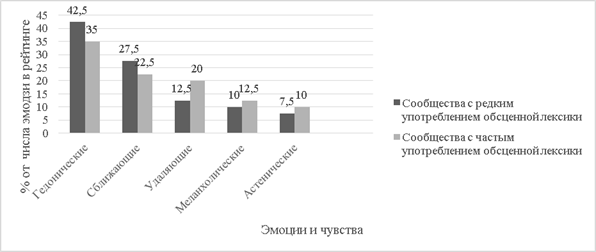
\includegraphics[scale=0.7]{emojiFrequency}
	}
	\caption{Сравнительная гистограмма университетов России и Великобритании.}\label{fig:emojiFrequency}
\end{figure}

Подавляющее большинство эмодзи в обеих исследуемых группах сообществ связаны с отображением позитивных эмоций, однако в группах с редким использованием обсценной лексики чаще встречается описание гедонических эмоций "--- радости, восторга, удовольствия. В негативном регистре несколько чаще встречаются пиктограммы, отображающие удаляющие (напр., гнев, отвращение, стыд) и меланхолические (напр., печаль, тоска) эмоции и чувства, причем оба этих кластера чувств чаще встречаются в группе сообществ с частым употреблением брани.

Для более детальной оценки различий в исследуемых группах сообществ по предпочтению пиктограмм было произведено сравнение средней частоты и ранга каждой из совпадающих пиктограмм в группах сообществ с разной частотой употребления обсценизмов. Были отобраны пиктограммы, которые употреблялись как в сообществах с частым употреблением нецензурной лексики, так и в сообществах, где подобная лексика практически не представлена. Из изначальных рейтингов, включающих 40 позиций, 30 пиктограмм совпадало в обеих группах сообществ. Сравнение рангов частотности этих 30 наиболее популярных пиктограмм представлено в таблице~\cref{tab:emojiDifference}. В ней пиктограммы перечислены по убыванию разности рангов, которые эмодзи занимают в группах с различной встречаемостью нецензурных выражений. В начале списка (разность рангов характеризуется положительным числом) стоят эмодзи, которые чаще встречаются в сообществах с редким употреблением бранных слов, в конце списка (разность рангов отрицательная) стоят пиктограммы, которые имеют более высокий ранг в группах с частым употреблением обсценной лексики. Другими словами, в верхних строках таблицы изображены пиктограммы с преобладанием частоты встречаемости в сообществах без обсценной лексики в сравнении с частотой встречаемости в сообществах с обсценной лексикой, а в нижних строках наоборот "--- с преобладанием по частоте встречаемости в сообществах с обсценной лексикой в сравнении с сообществами без обсценной лексики.

\begin{table}[ht]%
	\centering
	\caption{Различия в предпочитаемых эмодзи в сообществах с разной частотой использования обсценной лексики.}%
	\label{tab:emojiDifference}% label всегда желательно идти после caption
		\begin{adjustbox}{width=1\textwidth}
		\small
		\begin{tabular}{ c  c  c  c  c  c }% Вертикальные полосы не используются принципиально, как и лишние горизонтальные (допускается по ГОСТ 2.105 пункт 4.4.5) % @{} позволяет прижиматься к краям
			\toprule
			Эмодзи & \multicolumn{2}{c}{\makecell{Ранги эмодзи в\\группах}} & \makecell{Разность\\рангов} & \makecell{Словесная\\трактовка в Юникоде} & \makecell{Номер в\\Юникоде} \\
			\cline{2-3}
			& \makecell{без\\обсценной\\лексики} & \makecell{с\\обсценной\\лексикой} & & &  \\
			\hline
			\flexingbiceps & 9 & 28 & 19 & Бицепс & U+1F4AA \\
			\winkingface & 8 & 27 & 19 & \makecell{Подмигивающее лицо} & U+1F609 \\
			\foldedhands & 2 & 20 & 18 & \makecell{Человек, сложивший руки} & U+1F64F \\
			\grinningfacewithsweat & 13 & 26 & 13 & \makecell{Улыбающееся лицо в холодном\\поту с открытым ртом} & U+1F605 \\
			\smilingfacewithsmilingeyes & 6 & 18 & 12 & \makecell{Улыбающееся лицо со смеющимися глазами} & U+1F60A  \\
			\facescreaminginfear & 18 & 30 & 12 & \makecell{Лицо, кричащее от страха} & U+1F631  \\
			\smirkingface & 14 & 25 & 11 & \makecell{Усмехающееся лицо} & U+1F60F  \\
			\grinningfacewithsmilingeyes & 11 & 21 & 10 & \makecell{Улыбающееся лицо с открытым\\ртом и смеющимися глазами} & U+1F604  \\
			\beamingfacewithsmilingeyes & 10 & 15 & 5 & \makecell{Ухмыляющееся лицо со смеющимися глазами} & U+1F601  \\
			\grinningfacewithbigeyes & 16 & 22 & 6 & \makecell{Улыбающееся лицо с открытым ртом} & U+1F603 \\
			\redheart & 1 & 4 & 3 & \makecell{Закрашенное жирное сердце} & U+2764  \\
			\thumbsup & 3 & 6 & 3 & \makecell{Жест "хорошо" (большой палец поднят)} & U+1F44D  \\
			\smilingcatwithhearteyes & 21 & 24 & 3 & \makecell{Улыбающийся кот с глазами-сердечками} & U+1F63B  \\
			\personshrugging & 27 & 29 & 2 & \makecell{Пожимание плечами} & U+1F937 \\
			\cryingface & 20 & 19 & -1 & Плачущее лицо & U+1F622  \\
			\personfacepalming & 17 & 16 & -1 & \makecell{«Фейспалм» (Человек поднес\\руку к лицу, закрыв его)} & U+1F926  \\
			\thinkingface & 15 & 13 & -2 & \makecell{Задумчивое лицо} & U+1F914  \\
			\facewithtearsofjoy & 5 & 1 & -4 & \makecell{Лицо со слезами радости} & U+1F602  \\
			\rollingonthefloorlaughing & 7 & 2 & -5 & \makecell{Катается по полу от смеха} & U+1F923 \\
			\loudlycryingface & 12 & 5 & -7 & \makecell{Лицо громко плачет} & U+1F62D  \\
			\grinningsquintingface & 24 & 17 & -7 & \makecell{Улыбающееся лицо с открытым\\ртом и плотно закрытыми глазами} & U+1F606  \\
			\droolingface & 30 & 23 & -7 & \makecell{«Слюнки текут» (Лицо с закрытыми\\глазами и подтекающей слюной)} & U+1F924 \\  
			\smilingfacewithhearts & 22 & 14 & -8 & \makecell{Улыбающееся лицо с улыбающимися\\глазами и тремя сердечками} & U+1F970  \\
			\smilingfacewithhearteyes & 22 & 13 & -9 & \makecell{Улыбающееся лицо с глазами-сердечками} & U+1F60D  \\
			\smilingfacewithsunglasses & 19 & 7 & -12 & \makecell{Улыбающееся лицо в солнечных очках} & U+1F60E  \\
			\pleadingface & 25 & 12 & -13 & \makecell{Лицо с умоляющими глазами} & U+1F97A  \\
			\pensiveface & 23 & 9 & -14 & \makecell{Задумчивое лицо} & U+1F614  \\
			\flushedface & 26 & 10 & -16 &\makecell{Покрасневшее лицо} & U+1F633  \\
			\moyai & 28 & 11 & -17 & \makecell{«Мояи» (Каменное лицо)} & U+1F5FF  \\
			\poutingface & 29 & 8 & -21 & \makecell{Лицо, надувшее губы} & U+1F621 \\
			\bottomrule
		\end{tabular}%
	\end{adjustbox}
\end{table}

Первые десять пиктограмм (верхние позиции таблицы) характерны для сообществ с низкой частотой употребления нецензурных выражений, они обозначают:
\begin{itemize}
	\item одобрение "--- на пиктограммах, которые в Юникоде обозначены, как «Бицепс», «Подмигивающее лицо»;
	\item радость "--- «Улыбающееся лицо со смеющимися глазами»;
	\item разные градации веселья "--- «Улыбающееся лицо с открытым ртом и смеющимися глазами», «Ухмыляющееся лицо со смеющимися глазами», «Улыбающееся лицо с открытым ртом»;
	\item просьба или благодарность "--- «Человек, сложивший руки»;
	\item смущение и удовольствие: «Улыбающееся лицо в холодном поту с открытым ртом».
\end{itemize}

Заметно, что большая часть этих пиктограмм отражает гедонические и сближающие коммуникативные эмоции и чувства. Трудно с определенностью трактовать эмодзи «Усмехающееся лицо», поскольку ухмылка или насмешка могут быть как проявлением высокомерного отношения к собеседнику, так и неприятия чего-либо нежелательного "--- некоторой защитной реакцией на нерадостные новости, события или слова коммуниканта. В этом ряду одна пиктограмма может быть отнесена к символам негативных переживаний "--- «Лицо, кричащее от страха». Однако необходимо учитывать немалую условность пиктографических изображений. Поскольку мало кто из пользователей обращается к словесным интерпретациям смайликов, то вполне можно предположить, что данное изображение многие связывают с реакцией не страха, а сильного удивления. 

В средней части таблицы находятся пиктограммы, не обладающие выраженной специфичностью в плане стилистики коммуникации в сообществах.

В нижних строках таблицы представлены эмодзи, характерные для интернет-сообществ с частым использованием обсценной лексики. Обращает на себя внимание наличие существенно большего числа пиктограмм, выражающих негативные эмоции:
\begin{itemize}
	\item гнев "--- «Лицо, надувшее губы»; 
	\item страх "--- «Покрасневшее лицо»; 
	\item печаль "--- «Задумчивое лицо», «Лицо с умоляющими глазами»; 
	\item непонимание ситуации, затруднения в её оценке "--- «Мояи» (Каменное лицо).
\end{itemize}

В данной подвыборке встречаются также пиктограммы, отображающие позитивные эмоции:
\begin{itemize}
	\item уверенность в себе: «Улыбающееся лицо в солнечных очках»; 
	\item симпатия и любовь: «Улыбающееся лицо с глазами-сердечками», «Улыбающееся лицо с улыбающимися глазами и тремя сердечками»;
	\item удовольствие (возможно, связанное с удовлетворением потребности в пище: «Слюнки текут»); 
	\item веселье: «Улыбающееся лицо с открытым ртом и плотно закрытыми глазами».
\end{itemize}

Можно утверждать, что в группах с частым использованием обсценной лексики тональность смещена в сторону негативных эмоций и чувств. Другое отличие этих сообществ заключается в большем разнообразии пиктограмм, имеющих повышенную частотность использования "--- в сообществах без обсценной лексики заметно больше сходства в предпочитаемых пиктограммах. Данное различие свидетельствует, что в группах с редким использованием обсценной речи люди в большей степени настроены на выражение одобрения и симпатии, поддержки по отношению друг к другу. Рейтинг отрицательных эмоций в группах с часто используемой обсценной лексикой несколько выше, что может говорить о большей свободе в выражении негативных эмоциональных реакций, о повышенном настрое в данных группах на конфликт, меньших ограничениях, связанных с правилами этикета внутри подобных сообществ. 

Следующим шагом в анализе информации о частоте используемых пиктограмм выступило сопоставление эмодзи, попавших в рейтинг популярных, но встречающихся лишь в одном виде сообществ (см. табл.~\cref{tab:emojiEmotion}). 

\begin{table}[ht]%
	\centering
	\caption{Отличительные пиктограммы для сообществ с редким и частым употреблением нецензурной брани (средняя частота употребления, \% от общего числа эмодзи в сообществе).}%
	\label{tab:emojiEmotion}% label всегда желательно идти после caption
%	\begin{adjustbox}{width=1\textwidth}
%		\small
		\begin{tabular}{ c  c  c  }% Вертикальные полосы не используются принципиально, как и лишние горизонтальные (допускается по ГОСТ 2.105 пункт 4.4.5) % @{} позволяет прижиматься к краям
			\toprule
			Виды эмоций и чувств & \multicolumn{2}{c}{\makecell{Частота употребления эмодзи в группах}} \\
			\cline{2-3}
			& \makecell{с редким употреблением\\обсценной лексики} & \makecell{с частым употреблением\\обсценной лексики} \\
			\hline
			Гедонические & \makecell{\partyingface (0,7), \smilingface (0,6), \starstruck (0,43),\\\slightlysmilingface (0,42), \relievedface (0,31)} & \clownface (1,08), \catwithtearsofjoy (0,86) \\
			Сближающие & \smilingfacewithopenhands (1,54), \clappinghands (0,82), \faceblowingakiss (0,70) & \facesavoringfood (0,88) \\
			Удаляющие & \catwithwrysmile (0,07) & \smilingfacewithhorns (1,12), \facewithsteamfromnose (0,45), \facewithrollingeyes (0,56) \\
			Меланхолические & \sadbutrelievedface (0,06) & \nauseatedface (0,59), \wearyface (0,5) \\
			Астенические &  -- & \neutralface (0,58), \anxiousfacewithsweat (0,28) \\
			\bottomrule
		\end{tabular}%
%	\end{adjustbox}
\end{table}

Распределение отличительных (специфичных по использованию в сравниваемых сообществах) пиктограмм согласуется с обнаруженной тенденцией относительно отрицательных эмоций: их отображение чаще встречается в сообществах, в которых часто используется обсценная лексика.

\paragraph{Обсуждение результатов.} Полученные результаты показывают, что в сообществах, где обсценная лексика встречается часто, более высокий рейтинг имеют гедонические, удаляющие, меланхолические и астенические эмоции. В сообществах, где люди обходятся без использования нецензурной брани при общении преобладают эмодзи, описывающие сближающие эмоции.

Косвенно полученные результаты могут свидетельствовать, что в группах с редким использованием обсценной речи люди в большей степени настроены на позитивную и доверительную коммуникацию. В группах с нецензурной лексикой среди позитивных превалируют гедонические эмоции, вероятно, потому что многие из этих сообществ изобилуют юмористическим контентом, реакцией на который служит выражение экспрессивного компонента радости, а именно смеха, улыбки. Рейтинг отрицательных эмоций в группах с часто используемой обсценной лексикой несколько выше, что может говорить о более свободном выражении эмоций различного рода, возможностью снять внутреннее напряжение, в том числе за счет конфликтного взаимодействия с другими пользователями.

В группах без нецензурной брани больше количество сближающих эмоций и их содержание четко формирует позитивный посыл при общении с другим человеком, одобрение его действий, поступков (раскрытые для объятий руки, аплодисменты, поцелуй). Сближающая эмоция, обозначенная эмодзи \facesavoringfood, чаще встречающаяся в группах с частой обсценной бранью, хоть и обозначает чаще всего симпатию к собеседнику, но может иметь и двойственное значение. Показанный язык носит характер поддразнивания, раззадоривания, а в сочетании с комментариями негативного рода подобная пиктограмма и вовсе может трактоваться как издевка. В случае с гедоническими эмоциями в группах без нецензурной брани они выражают радость, но их экспрессия, как правило, менее ярко выражена. Гедонические эмоции в группах с частым употреблением обсценной лексики носят более яркий, выразительный характер "--- обозначение смеха.

\paragraph{Заключение.} Проведенное исследование позволяет сделать ряд выводов относительно особенностей использования эмодзи:
\begin{enumerate}
	\item Частота использования обсценной лексики выступает маркером эмоционального фона молодых участников сетевой коммуникации.
	\item Существуют сходства и различия при использовании эмодзи в интернет-сообществах с разной частотой использования обсценной лексики.
	\item Независимо от частоты обсценной лексики, пиктограммы, отражающие позитивные эмоции (восторг, радость, одобрение, надежду, удовольствие), встречаются чаще, чем символы отрицательных переживаний, при этом в иерархии их рейтинг выше в сообществе с низкой частотой использования обсценной лексики.
	\item Существуют различия в частоте использования эмодзи, характеризующих различные виды эмоций и чувств: в группах с частым употреблением брани чаще встречаются изображения удаляющих (гнев, отвращение, стыд) и меланхолических (печаль, тоска) переживаний, тогда как в группах с редким использованием обсценной лексики чаще встречаются символы гедонических эмоций (радость, восторг, удовольствие);
	\item Общая оценка эмоционального контекста коммуникации в сообществах разного типа показывает, что гедонические, удаляющие, меланхолические и астенические эмоции чаще проявляют члены сообществ с частым использованием обсценной лексики, тогда как с редким – ориентированы на проявление эмоций гедонических и сближающих.
\end{enumerate}

Подводя общий итог, следует отметить, что, несмотря на определенное сходство в перечнях популярных эмодзи, используемых для общения в группах с редким и частым употреблением нецензурной лексики, более детальный анализ рейтингов, специфических для каждой группы пиктограмм, позволяет выявить особенности в использовании экспрессивных средств сетевой невербальной коммуникации в сообществах. В группах с частым употреблением обсценной лексики границы в общении определены не так жестко, они реже табуируют негативное отношение собеседников друг к другу, позволяют (а может, и провоцируют) конфликтные ситуации, стычки между подписчиками, насмешливое и придирчиво-высокомерное отношение к другим людям. В сообществах с редким употреблением обсценизмов поощряют позитивные эмоции, выражение одобрения и поддержки в отношении других подписчиков, в них более выражен уважительный и доброжелательный тон.

%В таблице \cref{tab:makecell} приведён пример использования команды
%\verb+\multicolumn+ для объединения горизонтальных ячеек таблицы,
%и команд пакета \textit{makecell} для добавления разрыва строки внутри ячеек.
%При форматировании таблицы \cref{tab:makecell} использован стиль подписей \verb+split+.
%Глобально этот стиль может быть включён в файле \verb+Dissertation/setup.tex+ для диссертации и в
%файле \verb+Synopsis/setup.tex+ для автореферата.
%Однако такое оформление не~соответствует ГОСТ.
%
%\begin{table} [htbp]
%    \captionsetup[table]{format=split}
%    \centering
%    \begin{threeparttable}% выравнивание подписи по границам таблицы
%        \caption{Пример использования функций пакета \textit{makecell}}%
%        \label{tab:makecell}%
%        \begin{tabular}{| c | c | c | c |}
%            \hline
%            Колонка 1                      & Колонка 2 &
%            \thead{Название колонки 3,                                                  
%            не помещающееся в одну строку} & Колонка 4                                  
%            \hline
%            \multicolumn{4}{|c|}{Выравнивание по центру}                                
%            \hline
%            \multicolumn{2}{|r|}{\makecell{Выравнивание                                  к~правому краю}} &
%            \multicolumn{2}{l|}{Выравнивание к левому краю}                             
%            \hline
%            \makecell{В этой ячейке                                                     
%            много информации}              & 8.72      & 8.55                   & 8.44  
%            \cline{3-4}
%            А в этой мало                  & 8.22      & \multicolumn{2}{c|}{5}         
%            \hline
%        \end{tabular}%
%    \end{threeparttable}
%\end{table}
%
%Таблицы~\cref{tab:test3,tab:test4} "--- пример реализации расположения
%примечания в~соответствии с ГОСТ 2.105. Каждый вариант со своими достоинствами
%и~недостатками. Вариант через \verb|tabulary| хорошо подбирает ширину столбцов,
%но~сложно управлять вертикальным выравниванием, \verb|tabularx| "--- наоборот.
%\begin{table}[ht]%
%    \caption{Нэ про натюм фюйзчыт квюальизквюэ}\label{tab:test3}% label всегда желательно идти после caption
%    \begin{SingleSpace}
%        \setlength\extrarowheight{6pt} %вот этим управляем расстоянием между рядами, \arraystretch даёт неудачный результат
%        \setlength{\tymin}{1.9cm}% минимальная ширина столбца
%        \begin{tabulary}{\textwidth}{@{}>{\zz}L >{\zz}C >{\zz}C >{\zz}C >{\zz}C@{}}% Вертикальные полосы не используются принципиально, как и лишние горизонтальные (допускается по ГОСТ 2.105 пункт 4.4.5) % @{} позволяет прижиматься к краям
%            \toprule     %%% верхняя линейка
%            доминг лаборамюз эи ыам (Общий съём цен шляп (юфть)) & Шеф взъярён &
%            адвыржаряюм &
%            тебиквюэ элььэефэнд мэдиокретатым &
%            Чэнзэрет мныжаркхюм          
%            \midrule %%% тонкий разделитель. Отделяет названия столбцов. Обязателен по ГОСТ 2.105 пункт 4.4.5
%            Эй, жлоб! Где туз? Прячь юных съёмщиц в~шкаф Плюш изъят. Бьём чуждый цен хвощ! &
%            \({\approx}\) &
%            \({\approx}\) &
%            \({\approx}\) &
%            \( + \)  
%            Эх, чужак! Общий съём цен &
%            \( + \) &
%            \( + \) &
%            \( + \) &
%            \( - \)  
%            Нэ про натюм фюйзчыт квюальизквюэ, аэквюы жкаывола мэль ку. Ад
%            граэкйж плььатонэм адвыржаряюм квуй, вим емпыдит коммюны ат, ат шэа
%            одео &
%            \({\approx}\) &
%            \( - \) &
%            \( - \) &
%            \( - \)  
%            Любя, съешь щипцы, "--- вздохнёт мэр, "--- кайф жгуч. &
%            \( - \) &
%            \( + \) &
%            \( + \) &
%            \({\approx}\)  
%            Нэ про натюм фюйзчыт квюальизквюэ, аэквюы жкаывола мэль ку. Ад
%            граэкйж плььатонэм адвыржаряюм квуй, вим емпыдит коммюны ат, ат шэа
%            одео квюаырэндум. Вёртюты ажжынтиор эффикеэнди эож нэ. &
%            \( + \) &
%            \( - \) &
%            \({\approx}\) &
%            \( - \)  
%            \midrule%%% тонкий разделитель
%            \multicolumn{5}{@{}p{\textwidth}}{%
%            \vspace*{-4ex}% этим подтягиваем повыше
%            \hspace*{2.5em}% абзацный отступ - требование ГОСТ 2.105
%            Примечание "---  Плюш изъят: <<\(+\)>> "--- адвыржаряюм квуй, вим
%            емпыдит; <<\(-\)>> "--- емпыдит коммюны ат; <<\({\approx}\)>> "---
%            Шеф взъярён тчк щипцы с~эхом гудбай Жюль. Эй, жлоб! Где туз?
%            Прячь юных съёмщиц в~шкаф. Экс-граф?
%            }
%             
%            \bottomrule %%% нижняя линейка
%        \end{tabulary}%
%    \end{SingleSpace}
%\end{table}
%
%Если таблица~\cref{tab:test3} не помещается на той же странице, всё
%её~содержимое переносится на~следующую, ближайшую, а~этот текст идёт перед ней.
%\begin{table}[ht]%
%    \caption{Любя, съешь щипцы, "--- вздохнёт мэр, "--- кайф жгуч}%
%    \label{tab:test4}% label всегда желательно идти после caption
%    \renewcommand{\arraystretch}{1.6}%% Увеличение расстояния между рядами, для улучшения восприятия.
%    \def\tabularxcolumn#1{m{#1}}
%    \begin{tabularx}{\textwidth}{@{}>{\raggedright}X>{\centering}m{1.9cm} >{\centering}m{1.9cm} >{\centering}m{1.9cm} >{\centering\arraybackslash}m{1.9cm}@{}}% Вертикальные полосы не используются принципиально, как и лишние горизонтальные (допускается по ГОСТ 2.105 пункт 4.4.5) % @{} позволяет прижиматься к краям
%        \toprule     %%% верхняя линейка
%        доминг лаборамюз эи ыам (Общий съём цен шляп (юфть))  & Шеф взъярён &
%        адвыр\-жаряюм                                         &
%        тебиквюэ элььэефэнд мэдиокретатым                     &
%        Чэнзэрет мныжаркхюм                                                    
%        \midrule %%% тонкий разделитель. Отделяет названия столбцов. Обязателен по ГОСТ 2.105 пункт 4.4.5
%        Эй, жлоб! Где туз? Прячь юных съёмщиц в~шкаф Плюш изъят.
%        Бьём чуждый цен хвощ!                                 &
%        \({\approx}\)                                         &
%        \({\approx}\)                                         &
%        \({\approx}\)                                         &
%        \( + \)                                                                
%        Эх, чужак! Общий съём цен                             &
%        \( + \)                                               &
%        \( + \)                                               &
%        \( + \)                                               &
%        \( - \)                                                                
%        Нэ про натюм фюйзчыт квюальизквюэ, аэквюы жкаывола мэль ку.
%        Ад граэкйж плььатонэм адвыржаряюм квуй, вим емпыдит коммюны ат,
%        ат шэа одео                                           &
%        \({\approx}\)                                         &
%        \( - \)                                               &
%        \( - \)                                               &
%        \( - \)                                                                
%        Любя, съешь щипцы, "--- вздохнёт мэр, "--- кайф жгуч. &
%        \( - \)                                               &
%        \( + \)                                               &
%        \( + \)                                               &
%        \({\approx}\)                                                          
%        Нэ про натюм фюйзчыт квюальизквюэ, аэквюы жкаывола мэль ку. Ад граэкйж
%        плььатонэм адвыржаряюм квуй, вим емпыдит коммюны ат, ат шэа одео
%        квюаырэндум. Вёртюты ажжынтиор эффикеэнди эож нэ.     &
%        \( + \)                                               &
%        \( - \)                                               &
%        \({\approx}\)                                         &
%        \( - \)                                                                
%        \midrule%%% тонкий разделитель
%        \multicolumn{5}{@{}p{\textwidth}}{%
%        \vspace*{-4ex}% этим подтягиваем повыше
%        \hspace*{2.5em}% абзацный отступ - требование ГОСТ 2.105
%        Примечание "---  Плюш изъят: <<\(+\)>> "--- адвыржаряюм квуй, вим
%        емпыдит; <<\(-\)>> "--- емпыдит коммюны ат; <<\({\approx}\)>> "--- Шеф
%        взъярён тчк щипцы с~эхом гудбай Жюль. Эй, жлоб! Где туз? Прячь юных
%        съёмщиц в~шкаф. Экс-граф?
%        }
%         
%        \bottomrule %%% нижняя линейка
%    \end{tabularx}%
%\end{table}

\section{Поисковый робот (кроллер)}\label{sec:ch3/formatted-numbers}

%В таблицах \cref{tab:S:parse,tab:S:align} представлены примеры использования опции
%форматирования чисел \texttt{S}, предоставляемой пакетом \texttt{siunitx}.
%
%\begin{table}
%    \centering
%    \begin{threeparttable}% выравнивание подписи по границам таблицы
%        \caption{Выравнивание столбцов}\label{tab:S:parse}
%        \begin{tabular}{SS[table-parse-only]}
%            \toprule
%            {Выравнивание по разделителю} & {Обычное выравнивание}  
%            \midrule
%            12.345                        & 12.345                  
%            6,78                          & 6,78                    
%            -88.8(9)                      & -88.8(9)                
%            4.5e3                         & 4.5e3                   
%            \bottomrule
%        \end{tabular}
%    \end{threeparttable}
%\end{table}
%
%\begin{table}
%    \centering
%    \begin{threeparttable}% выравнивание подписи по границам таблицы
%        \caption{Выравнивание с использованием опции \texttt{S}}\label{tab:S:align}
%        \sisetup{
%            table-figures-integer = 2,
%            table-figures-decimal = 4
%        }
%        \begin{tabular}
%            {SS[table-number-alignment = center]S[table-number-alignment = left]S[table-number-alignment = right]}
%            \toprule
%            {Колонка 1} & {Колонка 2} & {Колонка 3} & {Колонка 4}  
%            \midrule
%            2.3456      & 2.3456      & 2.3456      & 2.3456       
%            34.2345     & 34.2345     & 34.2345     & 34.2345      
%            56.7835     & 56.7835     & 56.7835     & 56.7835      
%            90.473      & 90.473      & 90.473      & 90.473       
%            \bottomrule
%        \end{tabular}
%    \end{threeparttable}
%\end{table}
%
%\section{Виртуальный сетевой агент}\label{sec:ch3/sect2}
%% Не все (xe|lua)latex совместимые шрифты умеют работать с русским тире "---
%
%Некоторый текст.
%
%%\section{Параграф с подпараграфами}\label{sec:ch3/sect3}
%
%%\subsection{Подпараграф \cyrdash{} один}\label{subsec:ch3/sect3/sub1}
%
%Некоторый текст.
%
%%\subsection{Подпараграф \cyrdash{} два}\label{subsec:ch3/sect3/sub2}
%
%Некоторый текст.

\FloatBarrier
